\section{Running examples\label{section:background-running-examples}}

This section introduces the two running examples that will be used throughout the thesis. Section \ref{subsection:background-train-system} introduces a simple train control system. Section \ref{subsection:background-meeting-scheduler} introduces the meeting scheduler \cite{Feather:1997}.

\subsection{A simple train control system\label{subsection:background-train-system}}

A simplified train control system will be used as running example for illustrating concepts and techniques throughout this thesis. The system is composed of a software train controller, actuators for doors and train acceleration, sensors and passengers. Through the actuators, the software controller controls operations like starting or stopping the train, opening or closing doors, and so on. A safety goal requires train doors to remain closed while the train is moving. If the train is not moving and the passenger presses the alarm button, the controller must open the doors immediately. If the train is moving and the passenger presses the alarm button, the controller must stop the train first and then open the doors. Typical agent interactions for the latter case are depicted in Fig.~\ref{image:train-scenario-all-agents}. The precise semantics of such scenario will be made clear in the following sections.

\begin{figure}\centering
\scalebox{0.75}{
  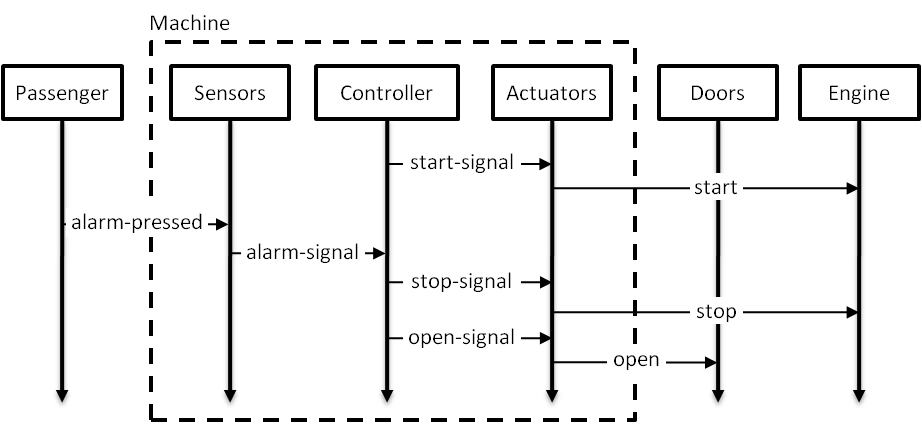
\includegraphics[trim=2mm 2mm 2mm 2mm, clip]{src/2-framework/images/train-scenario-all-agents}
}
\caption{A scenario illustrating a train system stopping in emergency when an alarm is pressed.\label{image:train-scenario-all-agents}}
\end{figure}

\subsection{The meeting scheduler\label{subsection:background-meeting-scheduler}}
